\documentclass[aspectratio=169, t]{beamer}

% 1. NO THEME: keep it completely barebones so the PPTX template can be applied later
\usetheme{default}
\usecolortheme{default}

% Disable navigation symbols and footlines to keep the bottom empty as requested
\setbeamertemplate{navigation symbols}{}
\setbeamertemplate{footline}{}

\usepackage{graphicx}
\usepackage{booktabs}
\usepackage{amsmath, amsfonts, amssymb}
\usepackage{caption}
\usepackage{subcaption}

\begin{document}

% ====== Frame 1: Title Page matching the image structure ======
\begin{frame}[plain]
    \vspace*{1cm}
    {\huge \textbf{Vision-Language-Action Models for Embodied Bimanual Manipulation in Industrial Environments}} \\[0.5cm]
    {\Large \textbf{Master's Thesis Defense}} \\[1cm]
    
    {\large Add optional group name} \\
    {\large Tian Qin, tian@xxxx.edu, Master's Program in EECS, Robotics Track} \\
    {\large If there is an additional author, add their email, programe code, and track.} \\[0.5cm]
    
    {\large Purpose: Master's Thesis Presentation} \\
    {\large Date: \today}
\end{frame}

% ====== Frame 2: Outline ======
\begin{frame}{Outline}
    \tableofcontents
\end{frame}

% ====== Frame 3: Introduction 1 ======
\begin{frame}{Introduction: The Rise of Embodied AI}
    \begin{itemize}
        \item Vision-Language-Action (VLA) models serve as the foundational brain for modern robotic systems.
        \item They bypass traditional modular pipelines (perception $\rightarrow$ planning $\rightarrow$ control).
        \item Instead, VLAs map high-dimensional multi-modal inputs (RGB cameras + text instructions) directly to low-level continuous joint actions.
        \item Despite these advances, the physical deployment of VLAs is heavily bottlenecked.
    \end{itemize}
\end{frame}

% ====== Frame 4: Introduction 2 ======
\begin{frame}{Core Challenges: The Deployment Gap}
    \begin{itemize}
        \item \textbf{Sim-to-Real Gap}: Many current VLA frameworks (e.g., OpenVLA, Octo) are heavily supervised on massive, low-quality Internet datasets or simulated environments. This causes severe failure rates in precise real-world tasks.
        \item \textbf{Bimanual Complexity}: Most existing VLAs focus on single-arm manipulation. Extending to two arms introduces exponential spatial and temporal coordination complexities.
        \item \textbf{High Inference Latency}: Large network backbones cause visual inference latency (100ms -- 500ms), inducing severe mechanical stuttering in the physical robots.
    \end{itemize}
\end{frame}

% ====== Frame 5: Objectives ======
\begin{frame}{Research Objectives}
    \begin{itemize}
        \item \textbf{Objective 1}: Construct a simulation-free, fully real-world bimanual robotic system capable of generating high-fidelity teleoperation data.
        \item \textbf{Objective 2}: Build an end-to-end framework integrating multi-view spatial awareness without depth sensors.
        \item \textbf{Objective 3}: Deploy and fine-tune continuous flow-matching VLA models ($\pi_0$ and $\pi_{0.5}$).
        \item \textbf{Objective 4}: Engineer an asynchronous system to strictly bind physical control latency under 50 ms.
    \end{itemize}
\end{frame}

% ====== Frame 6: Hardware - System Overview ======
\begin{frame}{Hardware: Bimanual Teleoperation System}
    We built an embodied AI system guaranteeing sub-millimeter precision for data collection:
    \begin{itemize}
        \item \textbf{Actuators}: Dual AgileX Piper 6-DoF robotic manipulators.
        \item \textbf{End Effectors}: Symmetrical 1-DoF AgileX Pika Grippers (Total 14-DoF).
        \item \textbf{Teleoperation Suit}: Pika Data Suit using 4 spatial base stations arrayed in a 45-degree opposing configuration to eliminate tracking occlusions.
        \item \textbf{Sampling Rate}: Hard-capped at 50 Hz for Cartesian mapping.
    \end{itemize}
\end{frame}

% ====== Frame 7: Hardware - View Topology ======
\begin{frame}{Hardware: Multi-Camera Sensory Matrix}
    \begin{columns}
        \begin{column}{0.4\textwidth}
            To provide robust spatial awareness:
            \begin{itemize}
                \item \textbf{Global View}: Intel RealSense D435 evaluating macro positions.
                \item \textbf{Active Wrist Views}: Two Intel D405 cameras securely mounted on independent end-effectors.
                \item \textbf{Format}: RGB-only, synchronized at 30 Hz.
            \end{itemize}
        \end{column}
        \begin{column}{0.6\textwidth}
            \centering
            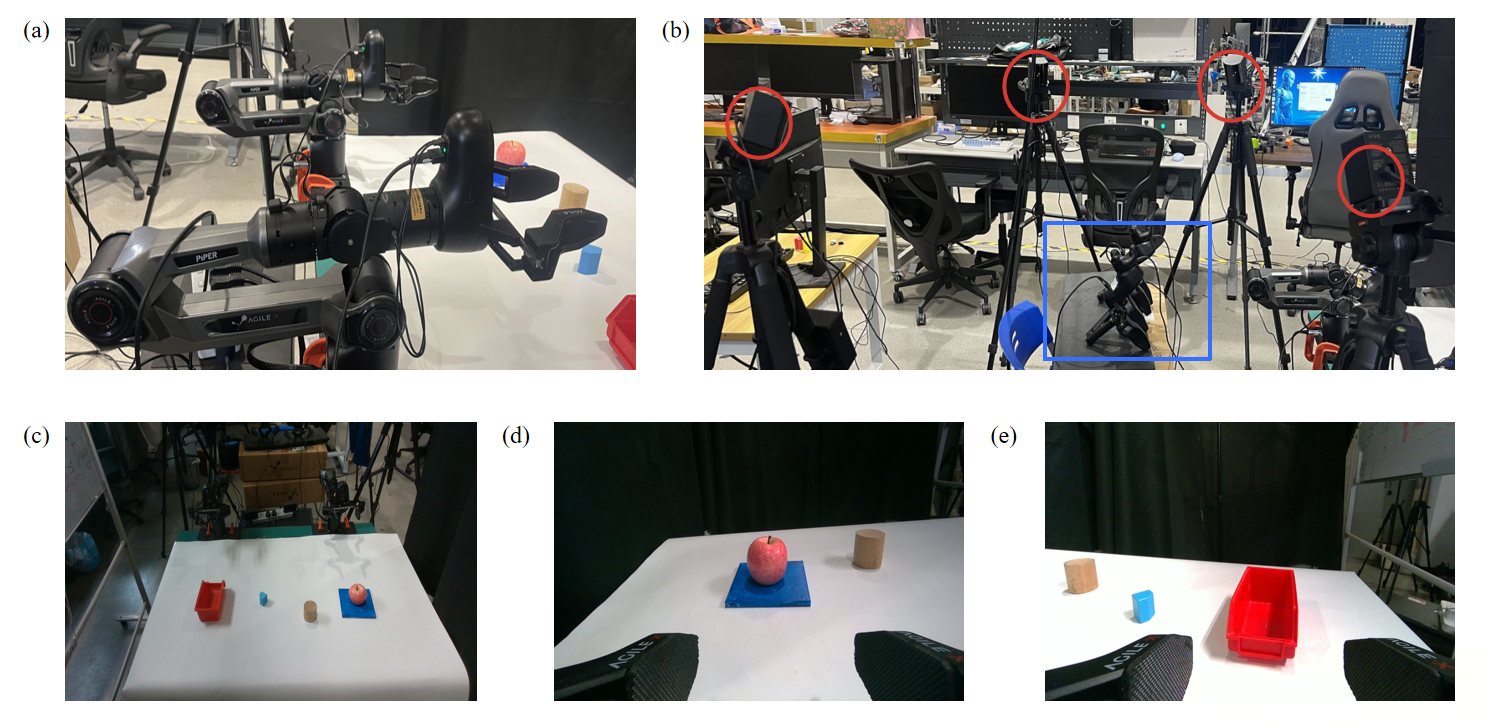
\includegraphics[height=0.7\textheight, keepaspectratio]{figures/3.1.png}
        \end{column}
    \end{columns}
\end{frame}

% ====== Frame 8: Task Definition ======
\begin{frame}{Task Formulation: Bimanual Apple Transfer}
    \begin{itemize}
        \item \textbf{Task Concept}: Move a target object (apple) from a starting board to a target bowl using sequential left-to-right bimanual handover.
        \item \textbf{Unique Constraints}:
        \begin{itemize}
            \item Requires sub-millimeter precision due to the narrow geometric clearance of the Pika Grippers.
            \item Real-time dynamic offset logic.
            \item Strict visual-motor alignment during the relay phase to prevent the object from shifting or dropping.
        \end{itemize}
    \end{itemize}
\end{frame}

% ====== Frame 9: Task Phases ======
\begin{frame}{Task: The 4 Temporal Phases}
    \begin{columns}
        \begin{column}{0.35\textwidth}
            \textbf{Execution Sequence:}
            \begin{itemize}
                \item[1] \textbf{Acquisition} (Left Arm)
                \item[2] \textbf{Centering \& Evasion}
                \item[3] \textbf{Relay Extraction} (Right arm)
                \item[4] \textbf{Target Placement}
            \end{itemize}
        \end{column}
        \begin{column}{0.65\textwidth}
            \centering
            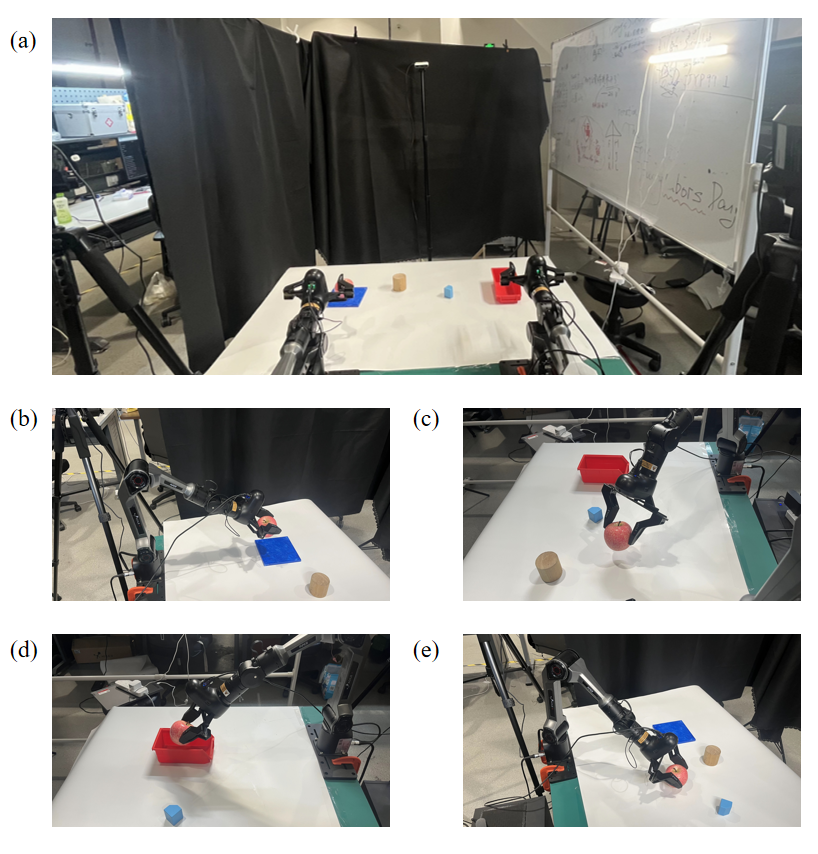
\includegraphics[width=\textwidth, height=0.7\textheight, keepaspectratio]{figures/3.2.png}
        \end{column}
    \end{columns}
\end{frame}

% ====== Frame 10: Data Protocol ======
\begin{frame}{Data Protocol: Quality Over Quantity}
    \begin{itemize}
        \item Traditional foundational models use \textit{millions} of generic trajectories.
        \item \textbf{Our approach}: Extreme data quality and absolute spatio-temporal alignment.
        \item We collected exactly \textbf{200 bimanual demonstrations} of the Apple Transfer task via expert human operators.
        \item \textbf{Temporal Master Clock}: Binds visual RGB frames against CAN bus kinematics timestamps to prevent phase divergence.
    \end{itemize}
\end{frame}

% ====== Frame 11: VLA Architecture (pi0) ======
\begin{frame}{VLA Architecture: $\pi_0$ Flow-Matching Baseline}
    \begin{columns}
        \begin{column}{0.5\textwidth}
            \begin{itemize}
                \item Adopted the 3B-parameter $\pi_0$ architecture by Physical Intelligence.
                \item Replaces discrete tokenized modeling with continuous Flow-Matching.
                \item Outputs precise continuous joint states natively.
            \end{itemize}
        \end{column}
        \begin{column}{0.5\textwidth}
            \centering
            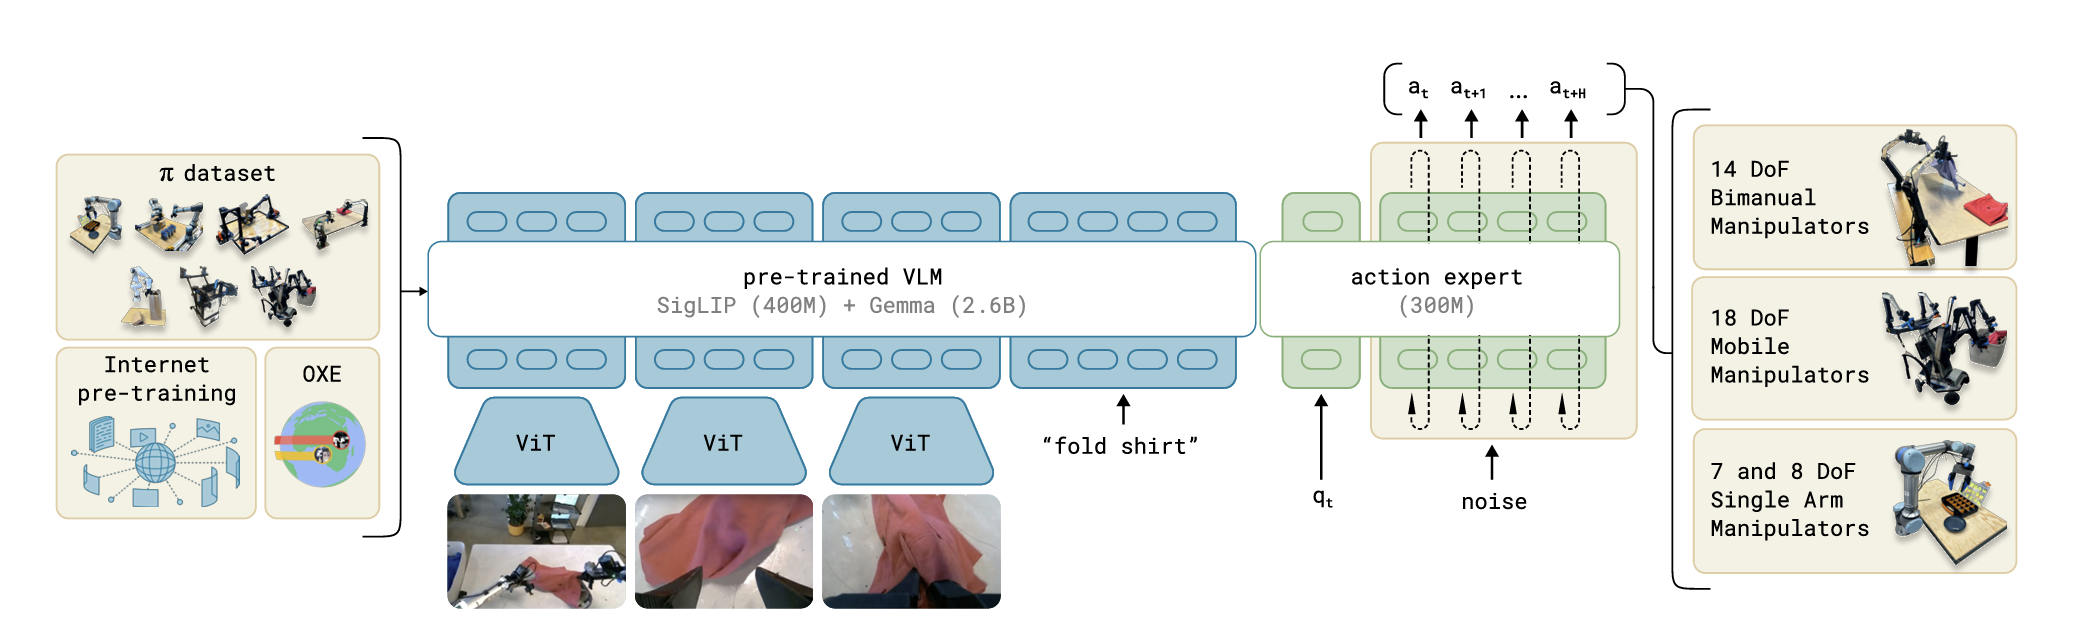
\includegraphics[width=\textwidth, height=0.7\textheight, keepaspectratio]{figures/pi0.png}
        \end{column}
    \end{columns}
\end{frame}

% ====== Frame 12: VLA Architecture (pi0.5) ======
\begin{frame}{VLA Upgrades: The $\pi_{0.5}$ Structure}
    \begin{itemize}
        \item Upgraded to the novel $\pi_{0.5}$ framework.
        \item \textbf{Quantile-Normalized Action Chunking}: Instead of single-step actions, the model predicts multi-step overlapping chunks.
        \item This exponentially increases temporal consistency and guards against single-frame camera noise.
        \item Directly supervised via L1 Flow error on the 200 real-world trajectories.
    \end{itemize}
\end{frame}

% ====== Frame 13: Deployment Bottlenecks ======
\begin{frame}{Deployment Constraints \& Execution Jitter}
    \begin{itemize}
        \item Large models ($\pi_0$ & $\pi_{0.5}$) introduce inference drag.
        \item On a standard RTX 4090 architecture, continuous generative flow integration scales up to 100~ms - 300~ms latency bounds.
        \item If pushed symmetrically to the robot controllers, this forces the hardware to vibrate destructively (mechanical jitter).
    \end{itemize}
\end{frame}

% ====== Frame 14: Asynchronous Client-Server ======
\begin{frame}{Solution: Asynchronous Client-Server Architecture}
    \begin{itemize}
        \item Decoupled high-level cognition from low-level execution logic.
        \item \textbf{Server Side}: Handles the GPU-intensive flow matching models visually.
        \item \textbf{Client Side}: Receives Chunk predictions asynchronously.
        \item \textbf{EMA Smoothing Factor}: Integrates Exponential Moving Average across the predicted action overlapping chunks.
        \item Execution instruction latency safely restricted below \textbf{50 ms}.
    \end{itemize}
\end{frame}

% ====== Frame 15: Latency Profiling ======
\begin{frame}{Latency Profiling Results}
    \begin{center}
        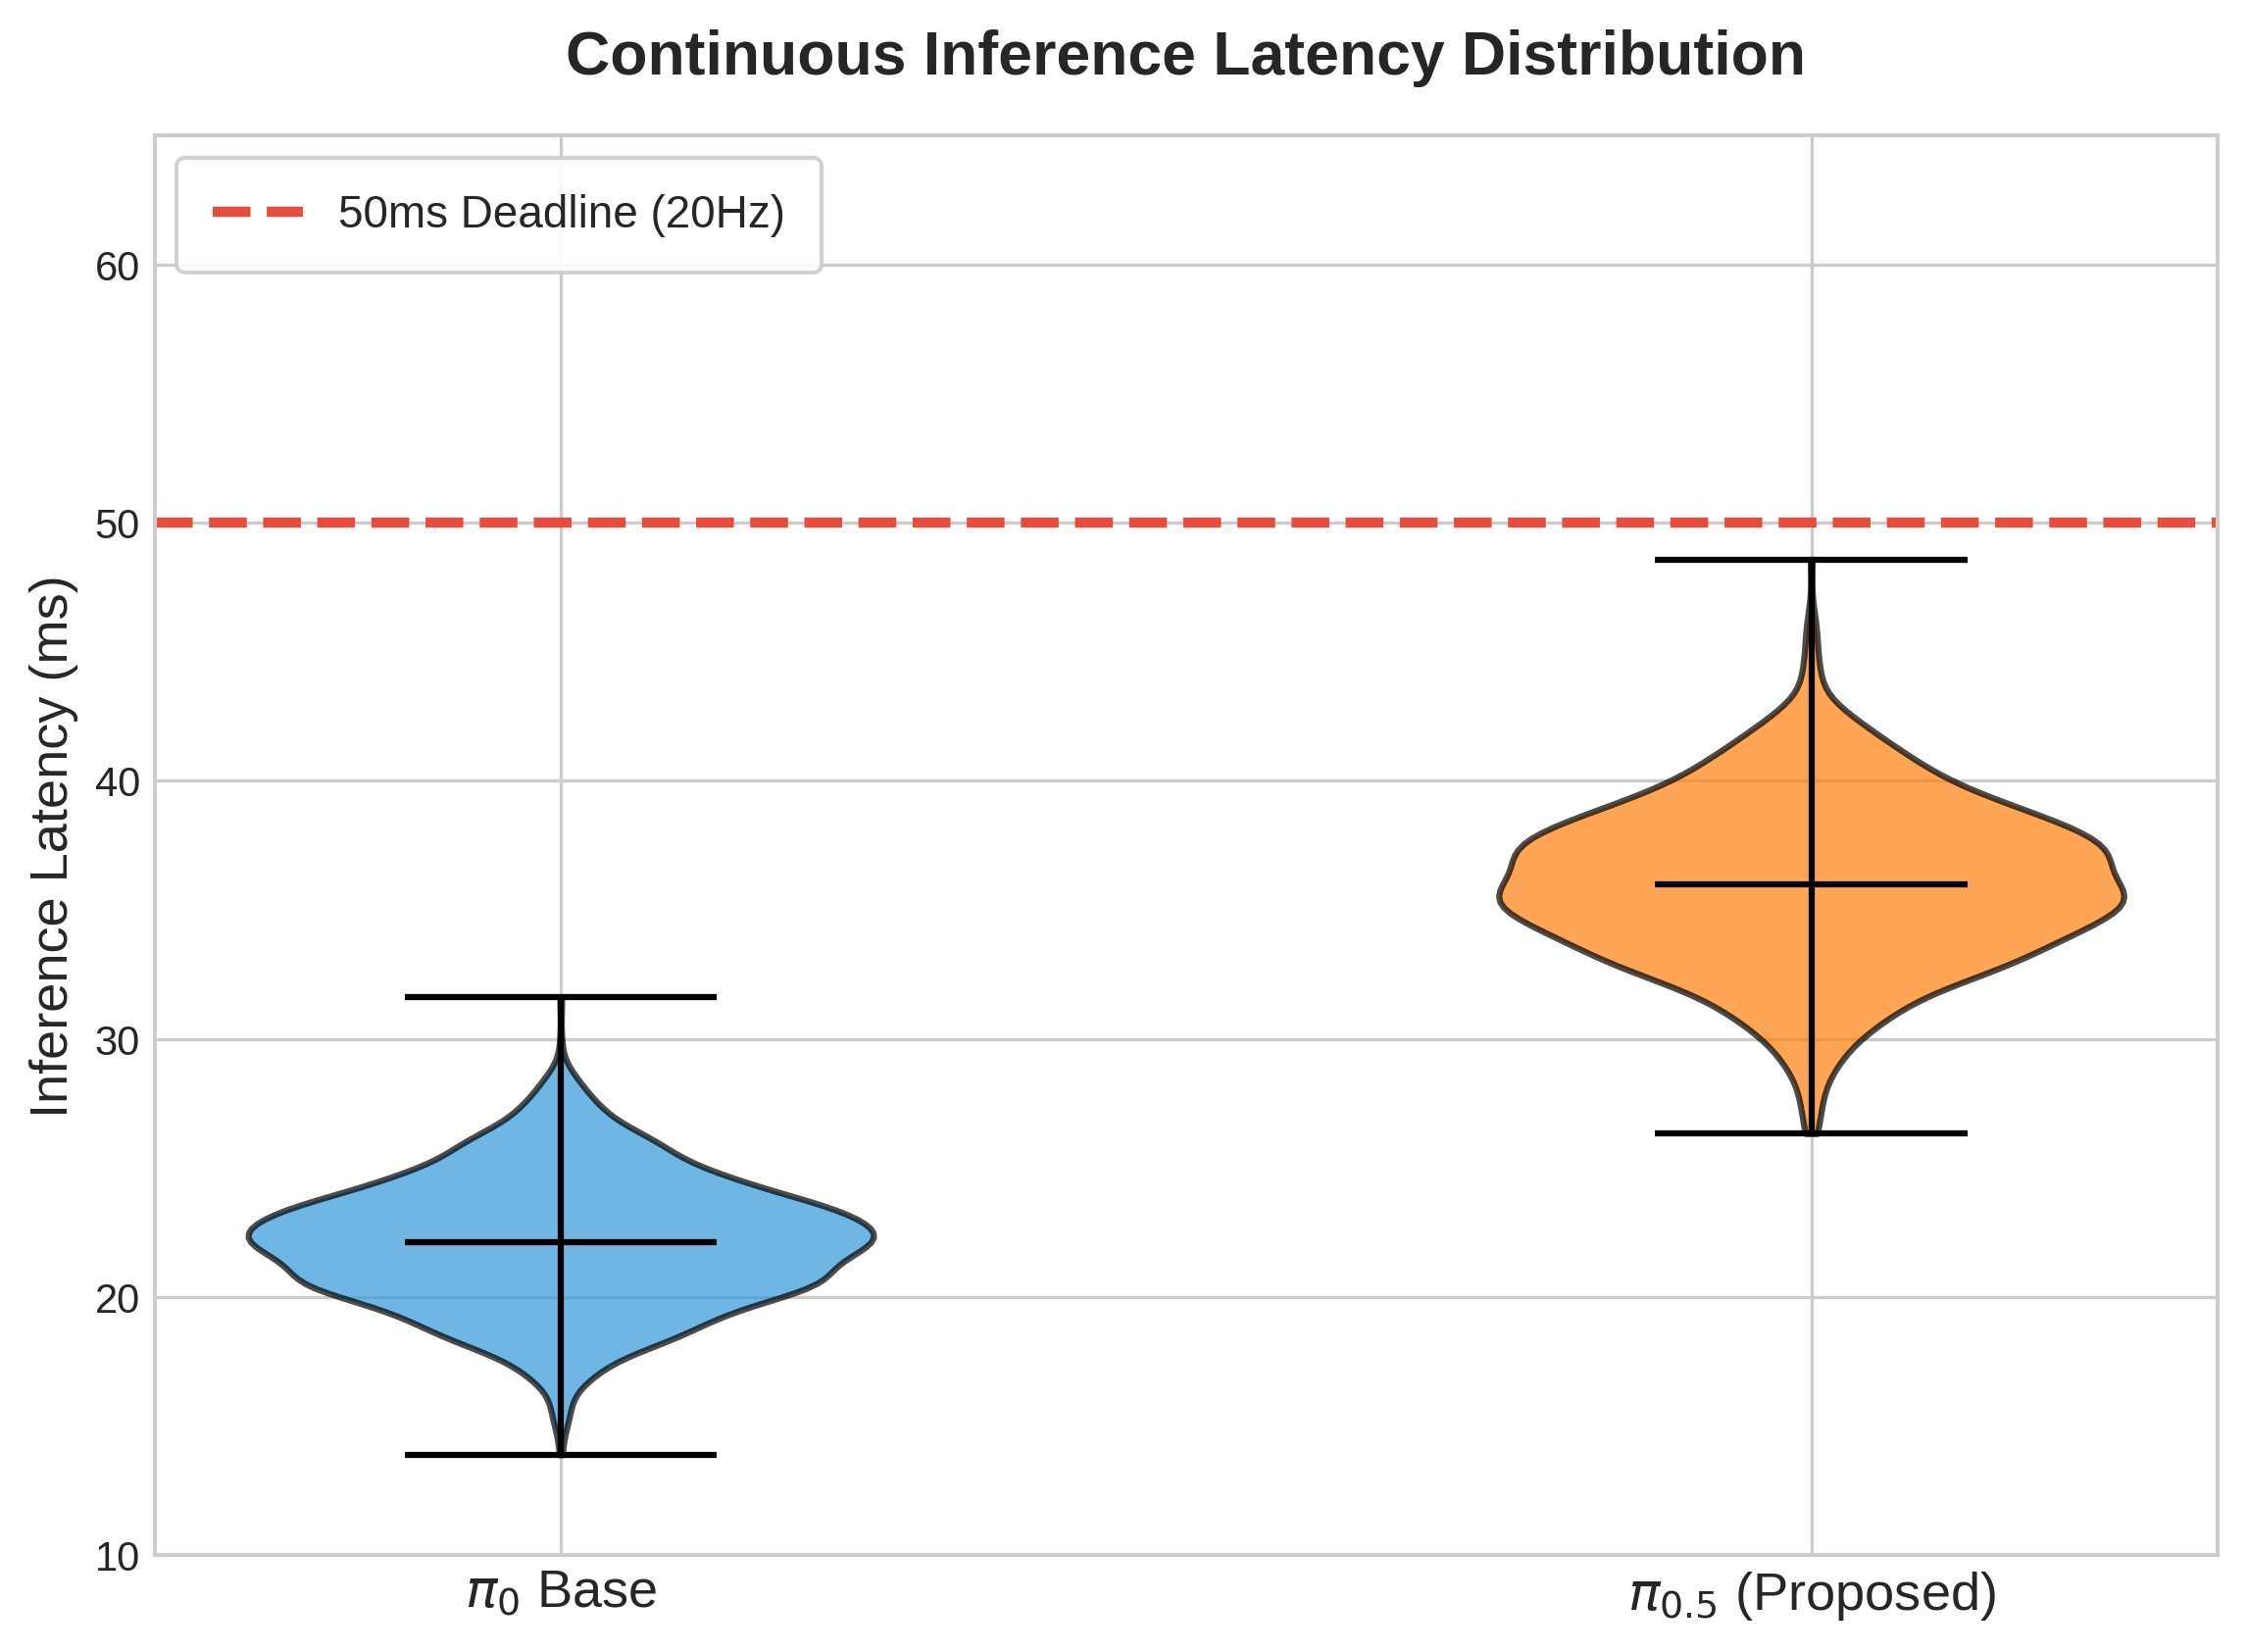
\includegraphics[width=0.85\textwidth, height=0.7\textheight, keepaspectratio]{figures/inference_latency.png}
    \end{center}
\end{frame}

% ====== Frame 16: End-to-End Success Rates ======
\begin{frame}{Evaluation: End-to-End Task Success Rates}
    \begin{itemize}
        \item We evaluated Zero-Shot base models vs. 200-demo Fine-Tuned (FT) models.
    \end{itemize}
    \begin{center}
        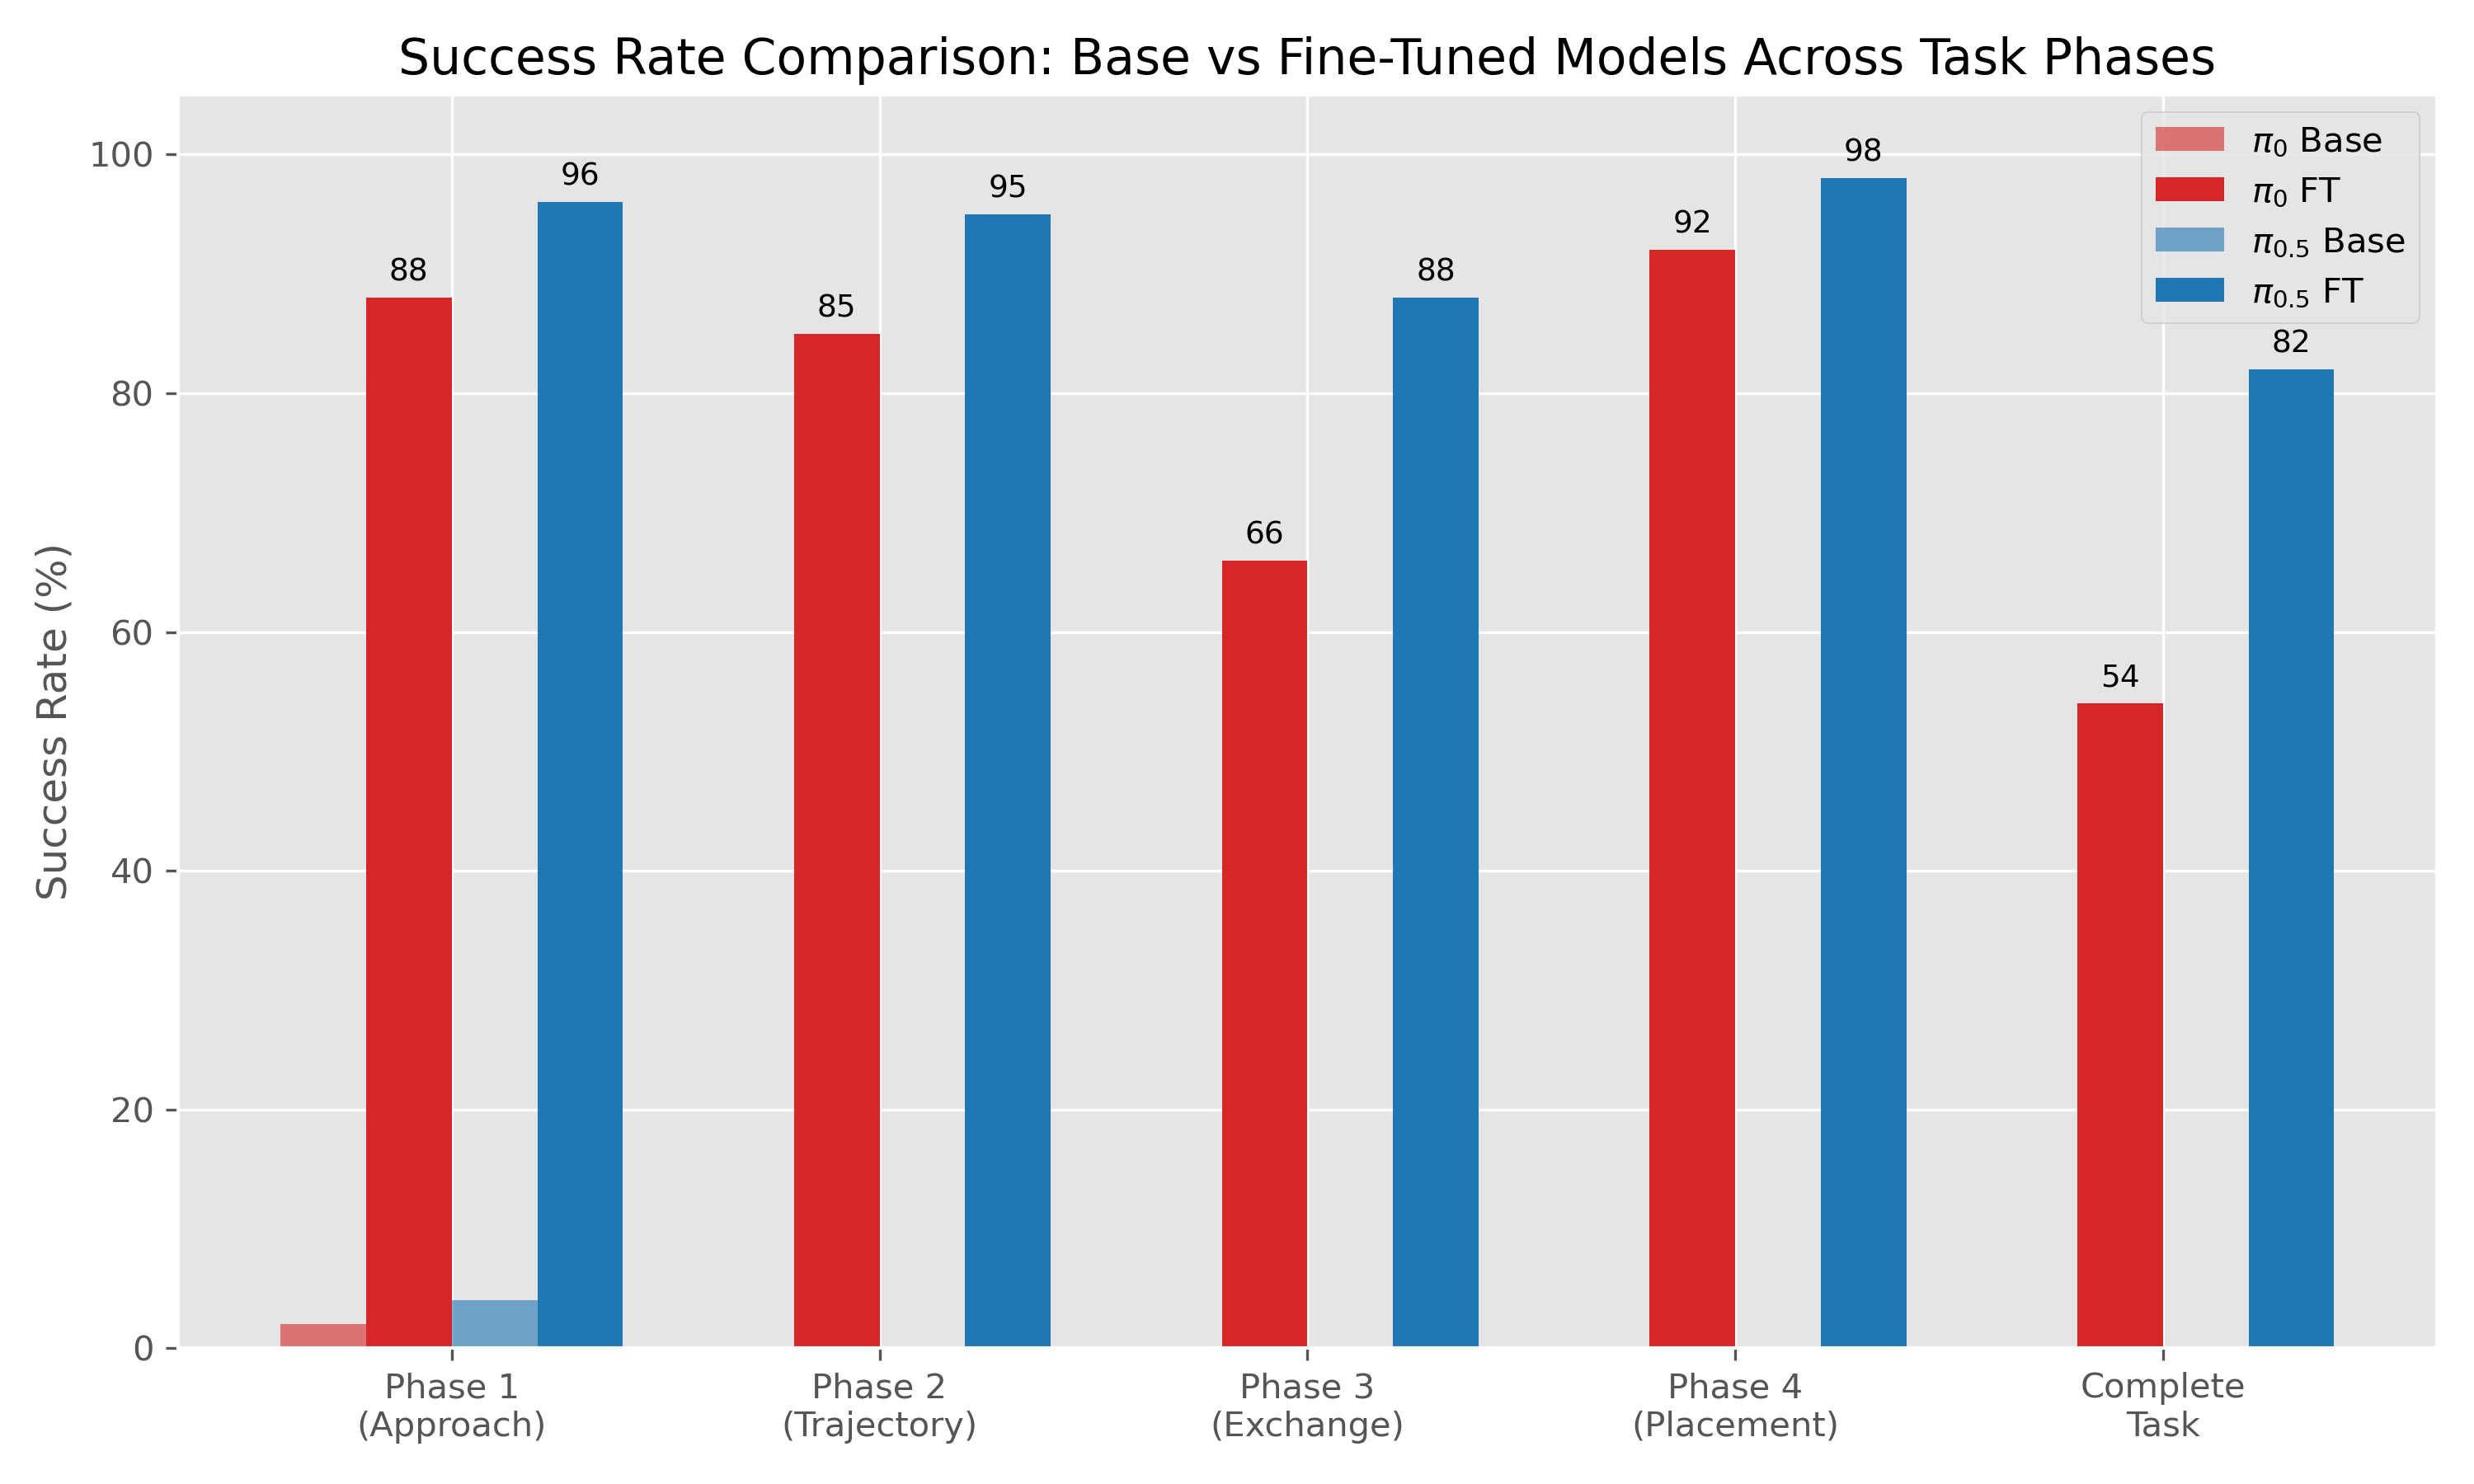
\includegraphics[width=0.85\textwidth, height=0.6\textheight, keepaspectratio]{figures/success_by_phase.png}
    \end{center}
\end{frame}

% ====== Frame 17: Evaluation Deep-Dive ======
\begin{frame}{Evaluation Insights}
    \begin{itemize}
        \item \textbf{Base Models Failure}: Both $\pi_0$ and $\pi_{0.5}$ pre-trained (Base) models recorded 0\% completion. They lack the sub-millimeter structural reasoning required for hardware-specific tasks.
        \item \textbf{Effectiveness of FT}: The Fine-Tuned versions reached remarkable task execution rates safely.
        \item \textbf{$\pi_{0.5}$ Superiority}: By chunking actions, $\pi_{0.5}$ FT smoothed out the handover relay inconsistencies effectively compared to the single-step $\pi_0$.
    \end{itemize}
\end{frame}

% ====== Frame 18: Loss Convergence \& Validation ======
\begin{frame}{Training Dynamics: Loss Convergence}
    \begin{columns}
        \begin{column}{0.4\textwidth}
            \begin{itemize}
                \item Strong convergence mapped via L1 Flow-Matching Error.
                \item Validated across held-out target distributions without catastrophic overfitting.
            \end{itemize}
        \end{column}
        \begin{column}{0.6\textwidth}
            \centering
            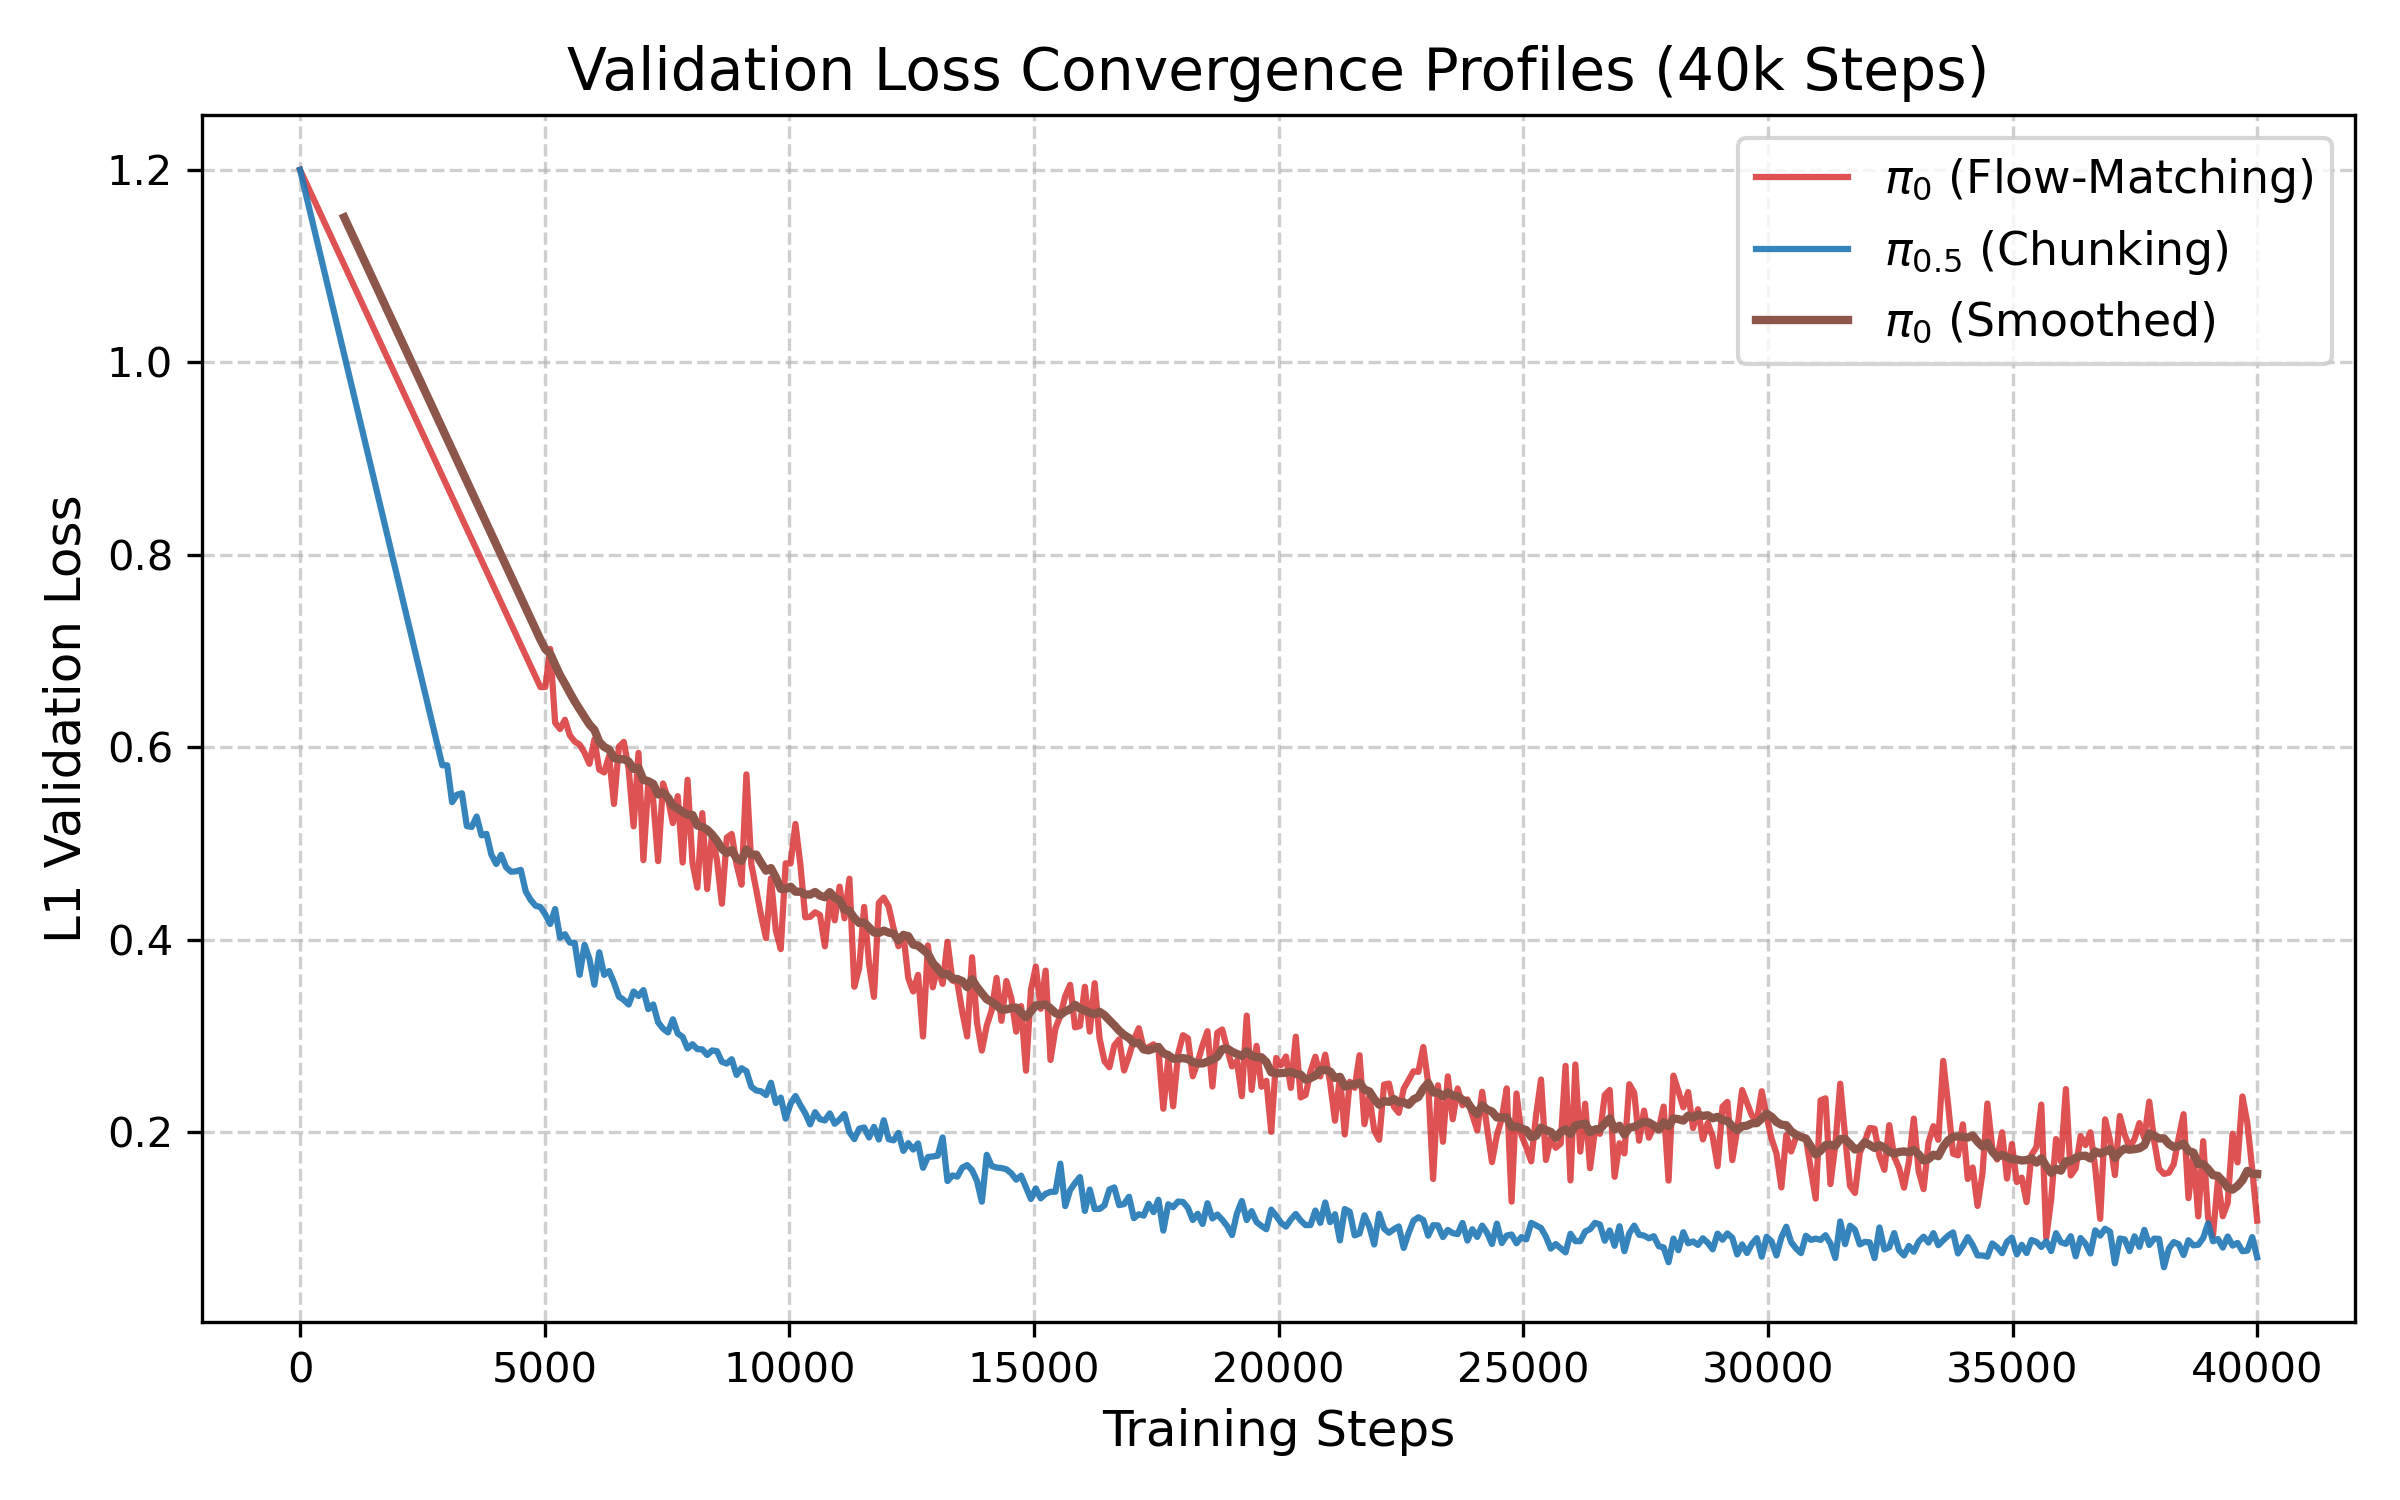
\includegraphics[height=0.7\textheight, keepaspectratio]{figures/val_loss_curves.png}
        \end{column}
    \end{columns}
\end{frame}

% ====== Frame 19: Offline Trajectory Alignment ======
\begin{frame}{Offline Kinematic Trajectory Alignment}
    \begin{center}
        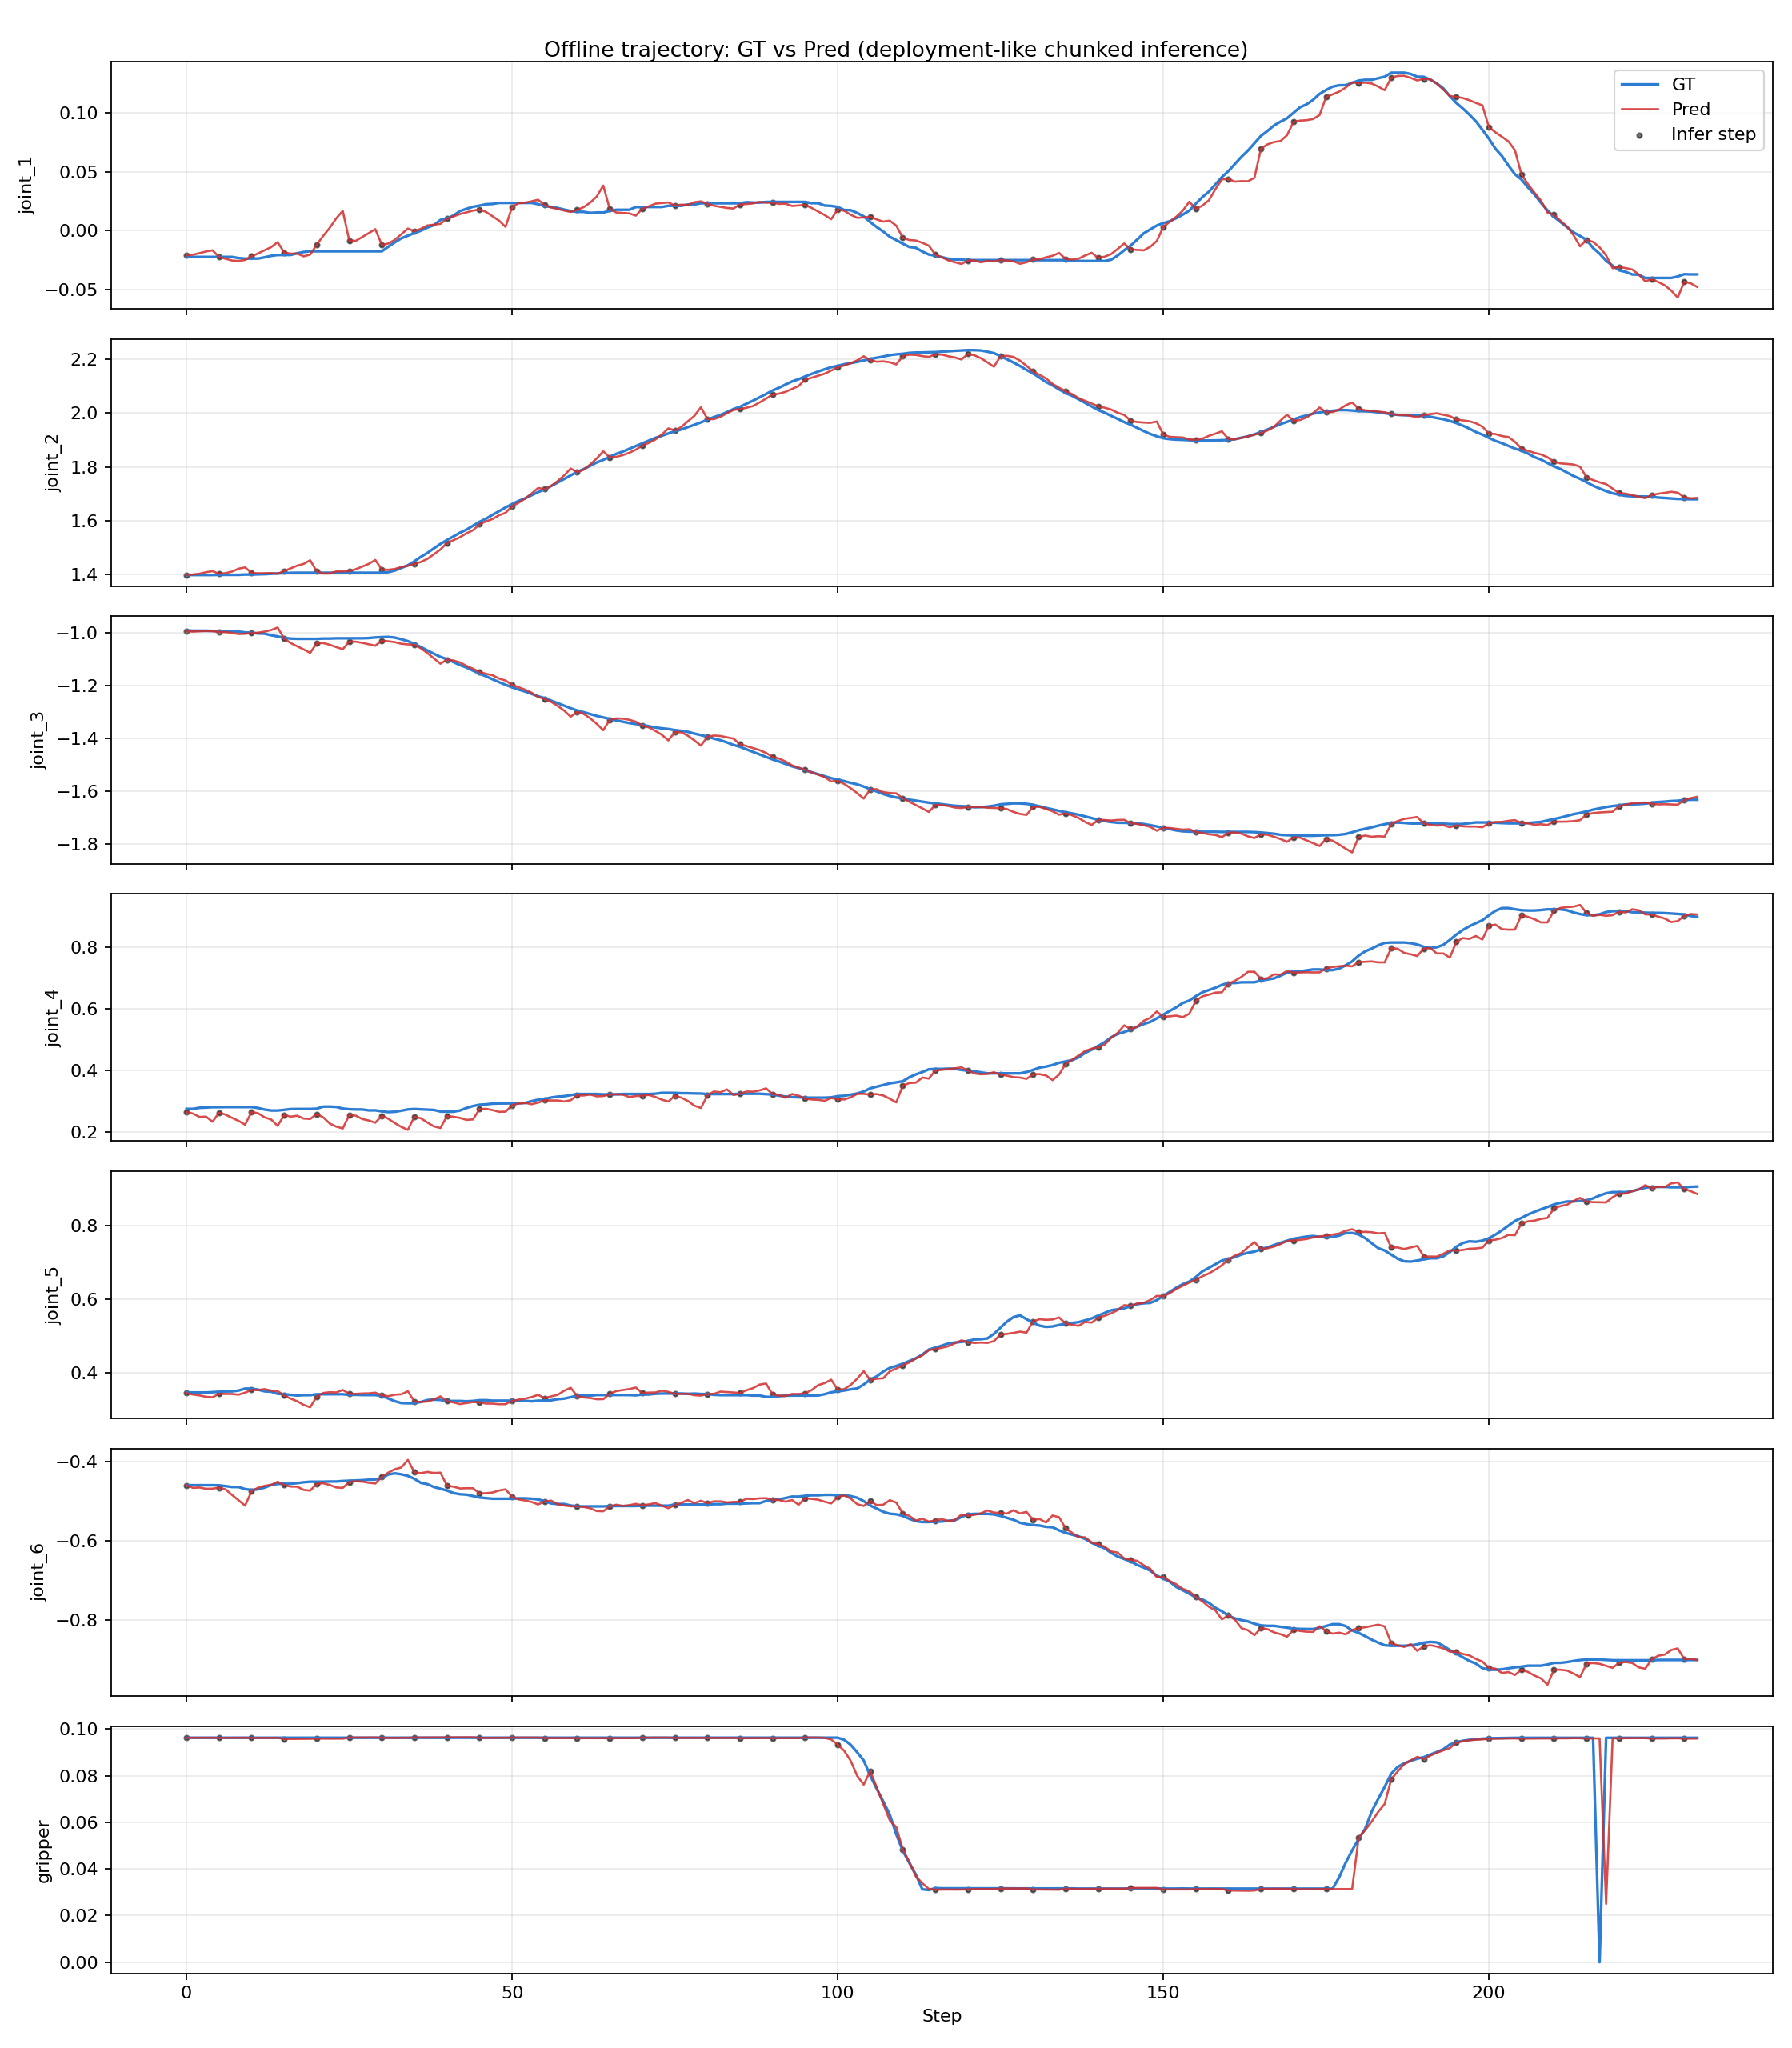
\includegraphics[width=0.9\textwidth, height=0.7\textheight, keepaspectratio]{figures/offline_trajectory_pi05.png}
    \end{center}
    \vfill
    \textit{The predicted spatial trajectories (orange) securely bind the underlying 14-DoF human operation vectors (blue).}
\end{frame}

% ====== Frame 20: Conclusion ======
\begin{frame}{Conclusions}
    \begin{itemize}
        \item Engineered a pure sim-free bimanual VLA pipeline on physical AgileX hardwares.
        \item Demonstrated that a \textbf{highly aligned, ultra-small dataset (200 trials)} is vastly superior to massive low-quality datasets for high-precision physical convergence.
        \item Solved the generation-lag paradox via Asynchronous Client-Server architecture and EMA action chunking ($\le 50$ms).
    \end{itemize}
\end{frame}

% ====== Frame 21: Future Work ======
\begin{frame}{Limitations \& Future Work}
    \begin{itemize}
        \item \textbf{Dynamic Robustness}: Explore zero-shot recovery behavior against external human perturbation.
        \item \textbf{Multi-modal integration}: Introduce force-feedback/tactile sensors to combat strict vision occlusion problems during cross-arm grasping.
        \item \textbf{Industrial Scaling}: Scale this dual-arm schema to standard industrial logistics scenarios.
    \end{itemize}
\end{frame}

% ====== Frame 22: Q&A ======
\begin{frame}[plain]
    \vspace*{2cm}
    \begin{center}
        \Huge \textbf{Thank You!} \\[1cm]
        \Large Questions \& Answers
    \end{center}
\end{frame}

\end{document}
